\documentclass[10pt,a4paper]{article}
\usepackage[T1]{fontenc}
\usepackage[utf8]{inputenc}
\usepackage{lmodern,microtype}
\usepackage[margin=17mm,top=17mm,bottom=18mm,headheight=14pt]{geometry}
\usepackage{amsmath,amssymb,booktabs,tabularx,array,multicol,xcolor}
\usepackage{graphicx,tikz,pgfplots,tcolorbox,enumitem,fancyhdr,titlesec,caption}
\usetikzlibrary{arrows.meta,positioning,shapes.geometric}
\pgfplotsset{compat=1.18}
\definecolor{navy}{HTML}{17334D}
\definecolor{teal}{HTML}{087F8C}
\definecolor{muted}{HTML}{596977}
\definecolor{pale}{HTML}{EDF5F6}
\definecolor{orange}{HTML}{C36B32}
\usepackage[colorlinks=true,urlcolor=teal,linkcolor=navy]{hyperref}
\hypersetup{pdftitle={BioPrint: Adaptive Behavioral Verification},pdfauthor={BioPrint},pdfsubject={Six-page research and implementation draft}}
\pagestyle{fancy}\fancyhf{}
\fancyhead[L]{\small\sffamily\bfseries\color{navy}BIOPRINT\quad\normalfont\small Research \& implementation}
\fancyhead[R]{\small\sffamily\color{muted}DRAFT FOR REVIEW}
\fancyfoot[L]{\scriptsize\color{muted}Dataset evidence \;\textbullet\; Synthetic policy evaluation \;\textbullet\; Working prototype}
\fancyfoot[R]{\small\thepage\,/\,6}
\renewcommand{\headrulewidth}{0.3pt}
\titleformat{\section}{\large\sffamily\bfseries\color{navy}}{\thesection}{0.6em}{}
\titleformat{\subsection}{\normalsize\sffamily\bfseries\color{teal}}{\thesubsection}{0.5em}{}
\titlespacing*{\section}{0pt}{10pt}{6pt}
\titlespacing*{\subsection}{0pt}{8pt}{4pt}
\setlength{\parindent}{0pt}\setlength{\parskip}{5pt}
\setlength{\tabcolsep}{4pt}\renewcommand{\arraystretch}{1.15}
\setlist{nosep,leftmargin=1.4em}
\captionsetup{font=small,labelfont=bf,skip=4pt,hypcap=false}
\newcommand{\note}[1]{\begin{tcolorbox}[colback=pale,colframe=teal,boxrule=0pt,leftrule=2pt,arc=0pt,left=7pt,right=7pt,top=5pt,bottom=5pt]#1\end{tcolorbox}}
\newcommand{\triple}[3]{#1 / #2 / #3}
\newcommand{\smalltable}{\fontsize{8.5}{10.4}\selectfont}
\begin{document}
\thispagestyle{fancy}
{\sffamily\color{teal}\small ACCOUNT-HOLDER VERIFICATION\par}
{\sffamily\bfseries\color{navy}\fontsize{28}{32}\selectfont BioPrint\par}
{\sffamily\color{navy}\Large Adaptive behavioral verification\par}
{\large From modality benchmarks to a working typing--pointer login\par}
\vspace{4pt}
\note{\textbf{Abstract.} BioPrint investigates whether browser interaction can help distinguish an account holder from an impostor who knows the password. We compare typing, pointer, device, bot, cognitive and touch signals; evaluate paired fusion and password-independent typing; and implement an adaptive login that prioritizes typing and requests pointer verification when needed. On a fixed synthetic cohort, integrating a trained pointer encoder changes false acceptance from \textbf{14/90 to 9/90}, while genuine rejection increases from \textbf{13/60 to 19/60}. These are policy-simulation results, not population accuracy estimates. The contribution is an instrumented prototype with explicit feature contracts, measured tradeoffs and reproducible evidence.}

\section{Introduction and background}
\subsection{The problem: a correct password is incomplete evidence}
A login form checks whether a secret is correct. The problem addressed here begins when an impostor already has that secret: can interaction with the form provide additional evidence about who is using it? A familiar device does not resolve a same-device attacker, while an unfamiliar device need not imply an unfamiliar person. BioPrint therefore separates three questions: \emph{Are the credentials valid? Does the interaction resemble automation? Does the behavior match the enrolled account holder?}

The intended outcome is a usable verification flow, not merely a classifier with a favorable average score. False acceptance admits an impostor; false rejection interrupts a legitimate user. A restrictive threshold can reduce the first error simply by rejecting almost everyone. Useful evaluation must expose both errors, the amount of interaction required and the availability of each signal.

\subsection{Landscape and positioning}
Behavioral fraud systems analyze patterns such as typing cadence, mouse movement and navigation. BioCatch describes physical and cognitive behavior analysis for detecting account takeover and other fraud [2]. This motivates the signal categories explored here; it does not establish equivalence with BioCatch's proprietary models or production performance. NIST distinguishes fraud indicators from authentication factors and recognizes behavioral biometric characteristics [1]. BioPrint is an experimental additional risk layer, not a demonstrated replacement for phishing-resistant authentication or a claim of standards compliance.

\begin{center}\small
\begin{tabularx}{\linewidth}{@{}p{29mm}XX@{}}
\toprule
\textbf{Evidence} & \textbf{What it contributes} & \textbf{What it cannot establish alone}\\\midrule
Credentials & Knowledge of the account secret & That the operator is its rightful owner\\
Browser/device context & Familiarity and changes in environment & Person identity on a shared or compromised device\\
Behavioral profile & Similarity to the account holder's interaction & Guaranteed identity across tasks, sessions or devices\\
Bot indicators & Scripted or mechanically repeated input & Complete resistance to adaptive automation\\\bottomrule
\end{tabularx}
\end{center}

\subsection{Scope of the work}
The investigation connects three levels of evidence: public-dataset benchmarks isolate signal quality; paired and synthetic experiments examine combinations; a browser application exercises enrollment, challenges and session decisions. The final prototype integrates an actual trained pointer encoder, while retaining an enrollment-based typing fallback for incompatible passwords. This report summarizes every experimental family; the accompanying \texttt{complete-results.csv} preserves individual variants, repeated controls and exact counts where available. Failed and infeasible experiments remain part of the evidence.

\newpage
\section{Final methodology: typing first, pointer when needed}
\subsection{Why this combination}
Typing is naturally available during password entry and requires no additional task. Source-dataset experiments favor nonlinear timing models, but strict low-FAR thresholds still reject many genuine attempts. Pointer verification supplies another behavioral observation without repeating the same typing evidence. In the four-policy synthetic comparison, statistical pointer step-up retained more genuine users than typing repetition, at the cost of more impostor accepts (Section 4). The SapiMouse study independently showed a substantial improvement over handcrafted pointer features. Together, these findings motivated the \emph{typing--pointer prototype}; they did not prove that it is universally optimal.

\begin{center}
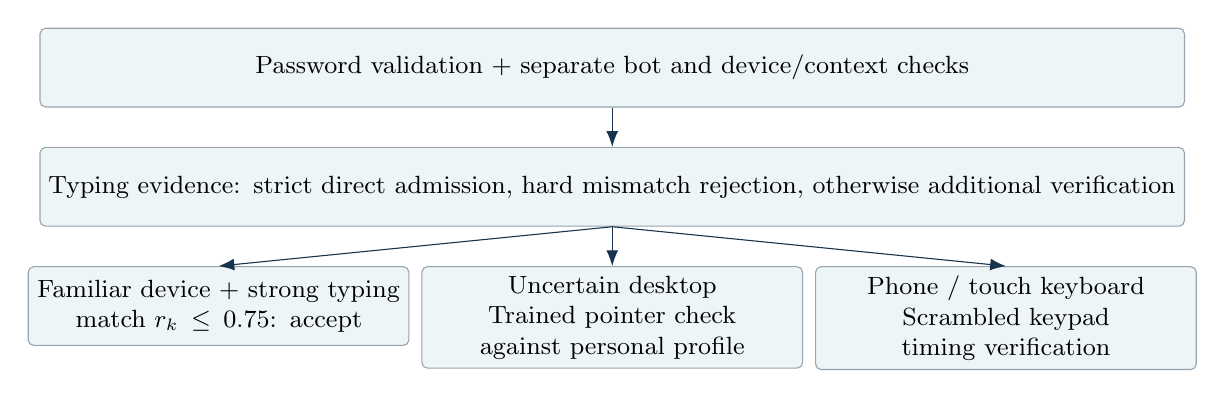
\begin{tikzpicture}[node distance=5mm and 8mm, every node/.style={font=\small},
 box/.style={draw=navy!45,fill=pale,rounded corners=2pt,align=center,text width=46mm,minimum height=10mm},
 arr/.style={-{Latex[length=2mm]},draw=navy}]
\node[box,text width=143mm] (input) {Password validation + separate bot and device/context checks};
\node[box,below=of input,text width=143mm] (typing) {Typing evidence: strict direct admission, hard mismatch rejection, otherwise additional verification};
\node[box,below=of typing,xshift=-50mm] (pass) {Familiar device +\ strong typing match\ $r_k\leq0.75$: accept};
\node[box,below=of typing] (desktop) {Uncertain desktop\ Trained pointer check\ against personal profile};
\node[box,below=of typing,xshift=50mm] (mobile) {Phone / touch keyboard\\ Scrambled keypad\\ timing verification};
\draw[arr] (input)--(typing);\draw[arr] (typing.south)--(pass.north);
\draw[arr] (typing)--(desktop);\draw[arr] (typing.south)--(mobile.north);
\end{tikzpicture}
\captionof{figure}{The principal enrolled-user flow. Failed credentials or bot checks block admission. Missing profiles invoke the existing enrollment/retyping fallback; absent evidence is not a match.}
\end{center}

\subsection{Typing and independent context checks}
Key events yield hold times $H_i=t_i^{\uparrow}-t_i^{\downarrow}$, down--down intervals $DD_i=t_{i+1}^{\downarrow}-t_i^{\downarrow}$ and up--down intervals $UD_i=t_{i+1}^{\downarrow}-t_i^{\uparrow}$. Negative $UD_i$ values capture overlapping presses. Personal enrollment uses one warmup and ten counted repetitions. A compatible feature schema enables an RBF SVM with separate TRAIN background examples ($C=10$, kernel-width factor $0.1$); other passwords use the personal scaled-distance scorer. The offline general typing models are \textbf{not deployed}.

Let $r_k=d_k/\tau_k$ be the typing score relative to its threshold. On a familiar device, $r_k\leq0.75$ permits direct admission; available typing above $2\tau_k$ blocks. Intermediate or missing evidence requests verification where an enrolled challenge exists. Browser context uses weighted attribute disagreement, not the researched FPStalker classifier. Bot indicators are separately evaluated and cannot be canceled by a favorable identity score.

\subsection{Trained pointer enrollment and verification}
Each desktop account records three one-minute mouse/trackpad sessions. Native coordinates and button events are preserved. Absolute coordinate displacements are standardized within 128-displacement blocks; a frozen fully convolutional encoder maps each block to a 128-dimensional embedding. The personal template is the normalized mean of normalized enrollment embeddings:
\[
 \hat z_j=\frac{z_j}{\|z_j\|_2},\qquad
 c_u=\frac{\sum_{j\in E_u}\hat z_j}{\|\sum_{j\in E_u}\hat z_j\|_2},\qquad
 s_p=\frac{1}{5}\sum_{j=1}^{5}\hat z_j^{\mathsf T}c_u .
\]
A challenge uses the first five complete blocks: 641 coordinates, without padding or joining sessions. Acceptance requires $s_p\geq0.948082149$, a frozen source-TRAIN threshold. The minimum duration is three seconds, but collecting enough points can take longer; source TRAIN median observation time was 16.89 seconds. This threshold is experimental for browser challenges. Nonces, expiry, account binding and exact-recording reuse checks protect the capture flow; client-reported trust alone is not tamper-proof attestation.

\subsection{Mobile behavior and implementation}
Mobile uses two scrambled-keypad runs against a cognitive timing profile built from six enrollment runs; desktop motor templates are not compared to thumb input. Mobile-only signup is not implemented. Current mobile policy accepts up to the full enrolled threshold ($r_c\leq1$), replacing the earlier $0.75$ multiplier. A flawed rule treating short inter-tap gaps as new visual searches was removed: the layout remains visible, so users can plan ahead. These changes have functional validation, \emph{not new FAR/FRR estimates}. FastAPI, SQLite and browser ES modules provide isolated databases, saved enrollment progress and signed sessions. An invitation-protected HTTPS gateway supports LAN testing. Profiles are not silently adapted after acceptance.

\newpage
\section{Experimental setup}
\subsection{Separate fitting, calibration and evaluation}
We distinguish population fitting, personal enrollment support, model selection, threshold calibration and DEV probes. For a distance score, acceptance is $d\leq\tau$; similarity scores reverse the inequality. Unless stated otherwise, source thresholds target empirical TRAIN-calibration FAR of 1\%. Evaluation reports the achieved DEV rates, which can exceed that target. Threshold selection follows the specified source protocol, rather than being inferred from a favorable DEV point.
\[
 \operatorname{FAR}(\tau)=\frac{N_{\mathrm{accepted\ impostor}}}{N_{\mathrm{impostor}}},\qquad
 \operatorname{FRR}(\tau)=\frac{N_{\mathrm{rejected\ genuine}}}{N_{\mathrm{genuine}}}.
\]
EER is the diagnostic point where FAR and FRR approximately coincide under a threshold sweep. It is not the FRR measured at a 1\% FAR target. CMU and the original KeyRecs comparisons report mean per-account EER; most other studies pool claims. These aggregations are not interchangeable. An application with several conditional gates has no prespecified single scalar sweep here, so \textbf{no app-wide EER is reported}.

\begin{center}\smalltable
\begin{tabularx}{\linewidth}{@{}p{31mm}p{59mm}X@{}}
\toprule
\textbf{Experiment family} & \textbf{Protocol / representation} & \textbf{Evaluation support}\\\midrule
CMU typing [3] & Ten session-1 enrollments; select on sessions 2--3, calibrate on 4, evaluate on 5--6 & 51 accounts; 100-enrollment study reported separately\\
KeyRecs typing & Session 1 split chronologically 50/25/25\% for fit/selection/calibration; session 2 DEV & Fixed: 79 accounts, 7,896 observations; free: 78 probe accounts, 4,525 windows\\
SapiMouse pointer & Five blocks per decision; separate personal support and DEV motion & 24 users; 76 genuine and 1,748 impostor comparisons\\
Context / bot / cognition & Pairwise browser linkage; held-out bot family; reaction-time/accuracy profiles & FPStalker: 154 browser IDs; DELBOT: 459 human/55 bot traces; cognition: 9 DEV people\\
Touch and paired sensing & TSI landing/timing; BEACON keyboard--pointer windows; HMOG typing--IMU & TSI: 12 people/356 trials; BEACON: 3 DEV people; HMOG: incomplete probe coverage\\
General typing & Identity-disjoint fit/calibration/evaluation; ten personal supports; pooled and single-source models & CMU: 28/13/10 identities; KeyRecs: 47/18/14; separate gameplay transfer\\
Four login policies & Same immutable cohort across four branches; real API and cookie checks in temporary databases & 39 artificial profiles, 390 scenarios per branch; DEV: 60 genuine/90 impostor\\\bottomrule
\end{tabularx}
\captionof{table}{Evaluation units differ by corpus. Neither window counts nor cross-account claim counts imply independent human trials.}
\end{center}

\subsection{Controlled combination experiments}
The four branches compare control, typing repetition, pointer step-up and cognitive keypad step-up. Each consumes the same hash-verified 12 TRAIN, 12 calibration and 15 DEV synthetic identities: 1,560 policy scenarios in total. Additional disjoint CMU identities supply typing background data. The original cohort combines real CMU typing with simulated target trajectories, timings, browser context and trust flags. It varies device familiarity, mobile input, genuine drift, scripts and owner-like typing/target attacks. Scenario weights are experimental choices, not estimated attack prevalence.

The trained-pointer follow-up preserves those 150 DEV cases and replaces desktop challenge data with native SapiMouse windows. Seed 20260920 maps 15 synthetic accounts to distinct source identities; their centers use separate three-minute support recordings. These are \textbf{artificial cross-dataset pairings}, not claims that the same real people appear in both datasets. Both policies run through the actual API and encoder from matched enrollment-only snapshots. One hundred alternative mappings test sensitivity to this assumption, without supplying new independent participants.

\subsection{Integrity, uncertainty and engineering checks}
Source hashes, frozen configurations, account/session roles and invalid-window counts accompany the experiments. Incorrect early synthetic fixtures and an overly restrictive pointer adapter are retained, rather than hidden. Some follow-up studies reused inspected DEV data; these are exploratory comparisons, not untouched-test confirmation. The final phone adjustments likewise follow live usability feedback.

For zero accepts in $n$ independent impostor trials, the one-sided 95\% upper bound is $1-0.05^{1/n}$: 72 trials imply 4.08\%, and at least 299 zero-error trials are needed to get below 1\%. Correlated claims weaken that interpretation. API parity checks establish implementation agreement, not biometric accuracy. Existing validations include 780,300 CMU score comparisons, 3,648 pointer scores and 6,241 short-capture Type2Branch scores. Browser checks exercise real event capture with mocked responses; isolated API replays separately exercise scoring and session issuance.

\newpage
\section{Results and interpretation}
\subsection{Individual modalities: improvements with explicit costs}
Table 2 compares the principal source-dataset methods. Each triple is \textbf{FAR / FRR / EER (\%)}; positive $\Delta$EER denotes an improvement. It compares methods \emph{within} protocols, not datasets against each other.
\begin{center}\smalltable
\begin{tabularx}{\linewidth}{@{}Xrrr@{}}
\toprule
\textbf{Dataset / task} & \textbf{Baseline} & \textbf{Candidate} & \textbf{$\Delta$EER (pp)}\\\midrule
CMU, 10 enrollments & 1.10 / 74.20 / 22.04 & 0.95 / 67.43 / 14.32 & +7.72 \\
CMU, 100 enrollments & 1.01 / 49.78 / 13.99 & 1.03 / 44.43 / 9.14 & +4.85 \\
KeyRecs fixed text & 1.26 / 76.39 / 17.08 & 1.29 / 45.91 / 11.62 & +5.46 \\
KeyRecs free text & 0.70 / 85.73 / 16.66 & 1.14 / 45.64 / 9.72 & +6.94 \\
SapiMouse, five blocks & 8.30 / 60.53 / 26.17 & 1.66 / 43.42 / 13.87 & +12.30 \\
FPStalker browser linkage & 0.69 / 8.33 / 3.79 & 0.84 / 4.85 / 2.30 & +1.49 \\
DELBOT bot geometry & 0.00 / 100.00 / 50.50 & 3.64 / 31.15 / 14.55 & +35.95 \\
Stroop/Flanker cognition & 1.39 / 88.89 / 48.61 & 2.78 / 77.78 / 27.78 & +20.83 \\
TSI touch landing & 1.00 / 95.51 / 36.75 & 1.00 / 91.85 / 34.45 & +2.30 \\
Balabit pointer & 1.89 / 98.20 / 48.61 & 1.93 / 92.45 / 56.18 & -7.58 \\
\bottomrule

\end{tabularx}
\captionof{table}{Source-dataset operating rates and diagnostic EER. FPStalker measures browser linkage; DELBOT measures bot versus human discrimination. Neither is account-holder verification.}
\end{center}

\begin{center}
\begin{tikzpicture}
\begin{axis}[width=.93\linewidth,height=45mm,xbar,bar width=5pt,xmin=0,xmax=30,
 ytick={0,1,2,3,4},yticklabels={CMU (10),CMU (100),KeyRecs fixed,KeyRecs free,SapiMouse},
 y dir=reverse,enlarge y limits=.17,xlabel={EER (\%) within each source protocol; lower is better},
 tick label style={font=\small},label style={font=\small},
 axis line style={draw=none},xmajorgrids,grid style={gray!15},
 legend style={at={(.99,.98)},anchor=north east,draw=none,font=\small}]
\addplot[fill=navy!35,draw=none,area legend] table[x=baseline,y=index]{eer-plot.dat};
\addplot[fill=teal,draw=none,area legend] table[x=candidate,y=index]{eer-plot.dat};
\legend{Baseline,Candidate}
\end{axis}
\end{tikzpicture}
\captionof{figure}{The main typing and pointer comparisons. The CMU 100-sample result has a different enrollment budget; the graph is not a cross-dataset ranking.}
\end{center}

\textbf{Typing.} CMU account-specific selection over nine RBF-SVM settings reduces EER by 7.72 pp versus scaled Manhattan; the paired-account bootstrap 95\% interval for new minus old EER is $[-11.11,-4.55]$ pp. Global SVM selection gives 1.00/72.98/15.50; explicitly minimizing TRAIN FRR at low FAR gives 0.99/64.10/18.50. The latter improves operating FRR but worsens EER. KeyRecs ExtraTrees replaces logistic regression on 47 fixed-text features or 35 summaries per 50 digraphs; FRR falls by 30.47 and 40.08 pp respectively.

\textbf{Pointer.} SapiMouse FCN--cosine reduces false accepts from 145 to 29 and false rejects from 46 to 33. Raw and enrollment-normalized one-class SVMs give 2.23/80.26/21.28 and 2.40/61.84/18.36. Z-normalized cosine gives 0.74/60.53/11.73: fewer false accepts, more genuine rejections. Its paired-bootstrap EER-difference interval, $[-5.47,+3.98]$ pp, includes zero; it was not selected by the TRAIN objective. Balabit ExtraTrees worsens pooled EER despite improving FRR and macro EER (38.30 to 30.09).

\textbf{Other modalities.} FPStalker histogram gradient boosting improves fuzzy browser linkage; exact equality yields 0/91.33/47.73. DELBOT random forest improves on a pointer-only rule reconstruction, which rejects every human; this does not evaluate the complete browser bot detector. Full Stroop/Flanker reaction-time and accuracy profiles outperform a single slope, but need hundreds of trials. TSI target-normalized random-forest features offer only modest touch gains. These findings support treating device context separately and deferring short cognitive tests as decisive identity evidence.

\subsection{Password-independent typing: implemented, evaluated, not promoted}
We trained logistic and ExtraTrees matchers using 42 summary-residual features, then tested 31 features derived from account-local positional alignment. Together, 54 model/dataset evaluations cover pooled fitting, single-source controls and cross-dataset/gameplay transfer (full ledger supplied). Summary-only pooled FRR is 98.80--99.90\% on CMU and 96.35--99.86\% on KeyRecs fixed. Aligned pooled logistic gives \textbf{0.42/95.30/25.41} and \textbf{3.83/88.98/29.42}; aligned trees give 1.72/90.90/24.19 and 4.58/82.61/30.78. Shipped-scorer EER on these smaller matched cohorts is 26.31 and 31.64. Improvements in separation do not offset these rejection rates. Only two fixed password texts are represented, and the aligned follow-up reuses DEV; neither model warrants universal-password accuracy claims.

\newpage
\subsection{Paired fusion and alternative experiments}
\textbf{BEACON tests genuine paired keyboard--pointer observations.} The matched comparison uses 140 windows from three DEV participants, producing 81 genuine and 162 impostor claims. All 81 windows shorter than 25 keystrokes remain included. Frozen encoders feed 24 balanced logistic candidates: eight feature combinations and $C\in\{0.01,0.1,1\}$. Separate TRAIN identity groups perform fitting, selection and calibration. Selection prioritizes FRR at a 1\% FAR constraint, then EER and $C$.

\begin{center}\small
\begin{tabularx}{\linewidth}{@{}Xrrrrr@{}}
\toprule
\textbf{Matched BEACON model} & \textbf{FA/162} & \textbf{FR/81} & \textbf{FAR} & \textbf{FRR} & \textbf{EER}\\\midrule
TypeNet & 0 & 81 & 0.00 & 100.00 & 35.80\\
SapiMouse & 108 & 46 & 66.67 & 56.79 & 59.26\\
Handcrafted behavior & 4 & 79 & 2.47 & 97.53 & 42.90\\
TypeNet + SapiMouse & 89 & 48 & 54.94 & 59.26 & 59.26\\
TypeNet + SapiMouse + handcrafted & 74 & 25 & 45.68 & 30.86 & 38.27\\
Type2Branch & 19 & 65 & 11.73 & 80.25 & 43.21\\
Type2Branch + SapiMouse & 105 & 48 & 64.81 & 59.26 & 59.26\\
Type2Branch + SapiMouse + handcrafted & 40 & 55 & 24.69 & 67.90 & 40.74\\\bottomrule
\end{tabularx}
\captionof{table}{Paired research fusion, rates in percent. ``All features'' here means available keyboard/pointer features, not all app signals. These are not synthetic-policy results.}
\end{center}

Replacing TypeNet with Type2Branch in the hybrid prevents 34 false accepts but creates 30 additional false rejects. FAR improves 20.99 pp; FRR worsens 37.04 pp; EER worsens 2.47 pp. At the observed operating point, balanced error rises from 38.27\% to 46.30\%. This is not evidence that a newer or more complex hybrid is automatically better. The separate general-typing transfer to BEACON gameplay is also weak: across nine frozen models, EER spans 48.91--55.19\%, with genuine rejection of 86.34--98.63\%.

\begin{center}\smalltable
\begin{tabularx}{\linewidth}{@{}p{48mm}p{37mm}X@{}}
\toprule
\textbf{Additional experiment} & \textbf{FAR / FRR / EER (\%)} & \textbf{Interpretation}\\\midrule
KeyRecs free, TypeNet transfer & 1.17 / 84.08 / 20.23 & Does not outperform feature-based ExtraTrees.\\
Type2Branch short capture & 9.14 / 30.38 / 13.93 & 79/79 accounts; 563/6,162 impostor accepts; different capture budget.\\
BEACON handcrafted fusion & 2.47 / 98.77 / 44.14 & Adding context gives 8.02 / 86.42 / 43.21.\\
BEACON nonlinear search & 2.47 / 98.77 / 43.83 & Retains logistic regression; EER convention changes, predictions do not.\\
BEACON neural-v1 fusion / hybrid & 41.98 / 34.57 / 39.51;\newline 2.47 / 98.77 / 43.21 & Early neural and handcrafted combinations; controls retained in ledger.\\
BEACON neural-v2 selected hybrid & 4.32 / 92.59 / 43.21 & Different selection from the matched hybrid in Table 3.\\
FPStalker RF / ThresholdFP adaptation & 0.80 / 5.27 / 2.38;\newline 1.12 / 7.99 / 3.97 & Browser-linkage alternatives; overlap score gives 1.21 / 33.08 / 7.57.\\
DELBOT logistic regression & 0.00 / 100.00 / 14.60 & Reject-all operating point despite lower diagnostic EER.\\
Cognitive means / learned RF & 0.00 / 100.00 / 31.94;\newline 4.17 / 88.89 / 30.56 & Neither beats the simpler full profile at a useful operating point.\\
HMOG joint / typing / IMU & 0.00 / 100.00 / 45.16;\newline 0.00 / 93.55 / 26.88;\newline 4.30 / 96.77 / 50.54 & Conditional on observed probes only; full-cohort validation fails.\\\bottomrule
\end{tabularx}
\captionof{table}{Alternative models and negative results. Complete per-variant rates, aggregation labels and source paths are in the companion ledger.}
\end{center}

\textbf{Coverage and infeasible studies.} Strict HMOG extraction yields 0/332 eligible windows. A frozen gap-filtered variant yields 207 windows but only 31/154 candidate genuine probes (20.13\%); two of four DEV people lack probes. Its joint model accepts none of the observed genuine probes. The touch extension has 77 support taps where 80 are required. Three-level arithmetic evaluates eight TRAIN candidates; the selected full-profile L1 model has 0/36 calibration false accepts and 11/12 false rejects. DEV is infeasible because one of 60 required blocks contains 50 rather than five entries. The original fixed-window Type2Branch protocol also lacks its required prefix. BrainRun establishes only a schema audit: 101 games, 982 gestures, seven of eight chosen users and six empty arrays. No recognition rates are assigned to these failures.

\textbf{What fusion mathematics permits.} For two required matches on a common population,
$\operatorname{FAR}_{\wedge}=P(A_k\cap A_p\mid I)$, not generally $\operatorname{FAR}_k\operatorname{FAR}_p$.
Conditional independence is unestablished, and unrelated datasets do not supply joint identities. Likewise, a three-level linear slope $b=(\bar t_3-\bar t_1)/2$ discards middle-level timing and accuracy. These observations explain why more signals, or a compact cognitive statistic, need direct validation rather than an assumed benefit.

\newpage
\subsection{End-to-end synthetic login comparison}
The original four-policy experiment compared shared scoring components and different decision paths; only compatible typing used the research-trained SVM. Its pointer/keypad challengers were statistical profiles. The neural follow-up then exercised the actual trained pointer encoder. The same 60 genuine and 90 impostor DEV cases underlie Table 5.
\begin{center}\small
\begin{tabularx}{\linewidth}{@{}Xrrrr@{}}
\toprule
\textbf{Policy / verification method} & \textbf{FA} & \textbf{FAR (\%)} & \textbf{FR} & \textbf{FRR (\%)}\\\midrule
Control & 32/90 & 35.56 & 5/60 & 8.33 \\
Typing repetition & 10/90 & 11.11 & 25/60 & 41.67 \\
Typing + statistical pointer & 14/90 & 15.56 & 13/60 & 21.67 \\
Typing + keypad & 13/90 & 14.44 & 16/60 & 26.67 \\
\textbf{Typing + trained pointer} & 9/90 & \textbf{10.00} & 19/60 & \textbf{31.67} \\
\bottomrule

\end{tabularx}
\captionof{table}{Final synthetic decisions after prescribed verification. All original candidates missed the 1\% calibration FAR gate; none earned automatic promotion to main.}
\end{center}

\begin{center}
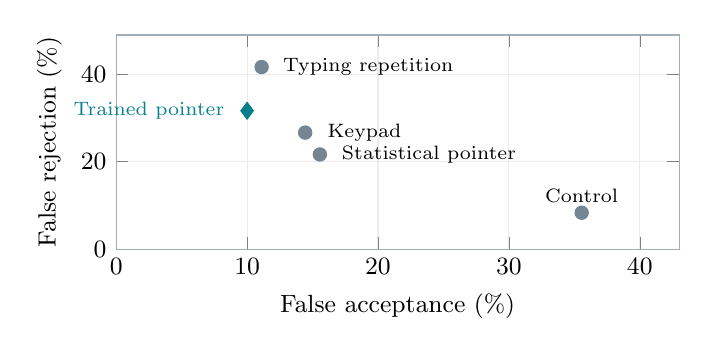
\begin{tikzpicture}
\begin{axis}[width=.72\linewidth,height=43mm,xmin=0,xmax=43,ymin=0,ymax=49,
 xlabel={False acceptance (\%)},ylabel={False rejection (\%)},
 tick label style={font=\small},label style={font=\small},grid=major,grid style={gray!15},
 axis line style={navy!40},clip=false]
\addplot[only marks,mark=*,mark size=2.4pt,color=navy!60] coordinates {(35.56,8.33) (11.11,41.67) (15.56,21.67) (14.44,26.67)};
\addplot[only marks,mark=diamond*,mark size=3pt,color=teal] coordinates {(10,31.67)};
\node[font=\scriptsize,anchor=south] at (axis cs:35.56,8.33){Control};
\node[font=\scriptsize,anchor=west] at (axis cs:12,41.67){Typing repetition};
\node[font=\scriptsize,anchor=west] at (axis cs:16.5,21.67){Statistical pointer};
\node[font=\scriptsize,anchor=west] at (axis cs:15.4,26.67){Keypad};
\node[font=\scriptsize,anchor=east,text=teal] at (axis cs:9,31.67){Trained pointer};
\end{axis}
\end{tikzpicture}
\captionof{figure}{Operating points, not an ROC curve. The lower-left direction is preferable; no scalar app EER follows from these policies.}
\end{center}

The trained-pointer replacement prevents \textbf{five false accepts} but adds \textbf{six genuine failures}: FAR improves 5.56 pp, FRR worsens 10.00 pp. Both paired variants request challenges in 63/150 cases, and the encoder decides 33 desktop cases. All 33 neural scores match frozen research predictions within $2\times10^{-6}$; cookie outcomes were checked across 300 paired API scenarios. An initial adapter incorrectly rejected 19 captures containing stationary points, producing 10.00\% FAR / 50.00\% FRR; preserving valid pauses fixes the adapter without changing the biometric threshold.

Source-calibrated thresholds targeting 0.1\%, 1\% and 5\% FAR give synthetic app FRR of 33.33\%, 31.67\% and 28.33\%, respectively, with FAR 10.00\% in all three counterfactuals. All nine residual false accepts bypass the encoder: seven owner-like typing attacks and two mobile keypad cases. Across 100 alternative identity mappings, FAR ranges 10.00--13.33\% and FRR 25.00--41.67\%; this is pairing sensitivity, not a confidence interval. At fixed observed counts, the substitution changes error cost by $-5c_{FA}+6c_{FR}$, favoring it when $c_{FA}/c_{FR}>1.2$, before prevalence and interaction costs.

\section{Conclusion}
BioPrint delivers an adaptive behavioral-verification prototype and a traceable path from signal benchmarking to live integration. The strongest practical finding is that trained pointer verification can reduce impostor acceptance among challenged cases, while typing preserves a low-friction direct path. The equally important finding is that routing governs the residual risk: improving a step-up model cannot detect an attacker who bypasses it.

The demonstrated result is a functioning research prototype, not validated population security. Current mobile threshold relaxation and the corrected bot rule postdate Table 5; \textbf{the latest live version has no newly measured aggregate FAR, FRR or EER}. Functional checks passed for pointer integration (41 tests), the bot correction (59) and mobile policy (32), in overlapping suites. Next validation should collect paired, consented multi-session users, freeze policy/calibration before evaluation, measure device-class coverage and capture burden, and test direct-admission attacks. Sensitive raw interaction records require a retention policy, and browser-reported events remain forgeable. These are concrete limits on deployment, not reasons to hide the measured gains.

\vspace{2pt}\hrule\vspace{3pt}
{\scriptsize\textbf{References and evidence.}
[1] NIST, \href{https://pages.nist.gov/800-63-4/sp800-63b.html}{SP 800-63B-4: Authentication and Authenticator Management}, Sections 2 and 3.
[2] BioCatch, \href{https://www.biocatch.com/what-we-do}{Behavioral biometrics and fraud detection}, official product overview.
[3] Killourhy and Maxion, \href{https://www.cs.cmu.edu/~keystroke/}{CMU Keystroke Dynamics Benchmark Data Set}.
[4] Repository evidence: \texttt{DATASET\_RESULTS.md}, general-typing result reports, and \texttt{NEURAL\_POINTER\_RESULTS.md}; full paths and SHA-256 hashes in \texttt{evidence-manifest.json}. All result variants are supplied in \texttt{complete-results.csv}. Live-method snapshot: \texttt{experiment/typing-pointer}, commit \texttt{f409a4d}.}
\end{document}
